\documentclass[a4paper,12pt]{report}
\usepackage{polski}
\usepackage[polish]{babel}
\usepackage[utf8]{inputenc}
\usepackage{lastpage}
\usepackage{fancyhdr}
\usepackage{titlesec}
\usepackage{listings}
\usepackage{color}
\usepackage{framed}
\usepackage{etoolbox}
\usepackage{graphicx}
\usepackage{indentfirst}
\usepackage{hyperref}
\hypersetup{
    colorlinks=true,
    linkcolor=black,
    filecolor=black,
    urlcolor=blue,
}

\urlstyle{same}

\makeatletter
\patchcmd{\@verbatim}
  {\verbatim@font}
  {\verbatim@font\small}
  {}{}
\makeatother

\titleformat{\chapter}
  {\normalfont\LARGE\bfseries}{\thechapter}{1em}{}
\titlespacing*{\chapter}{0pt}{0.5ex}{0.5ex}

\title{8mu \\ \large Specyfikacja implementacyjna}
\author{Krzysztof Piekarczyk \\ \small 288277}
\date{26 marca 2020}

\pagestyle{fancy}
\fancyhf{}
\rhead{Krzysztof Piekarczyk 288277}
\lhead{8mu: Specyfikacja implementacyjna}
\rfoot{Strona \thepage \space z \pageref{LastPage}}

\begin{document}
\maketitle

\tableofcontents
\thispagestyle{fancy}

\chapter{Wstęp}
\thispagestyle{fancy}
Celem tego dokumentu jest opisanie implementacji funkcjonalności programu ,,8mu'' opisanych w specyfikacji funkcjonalnej oraz opisu działań i narzędzi użytych w procesie implementacji.

\chapter{Środowisko deweloperskie}
\thispagestyle{fancy}
\section{Software}
\begin{itemize}
    \item System operacyjny: Windows 10
    \item Język programowania: C++11
    \item CLion 2019.3
    \item GCC-6.3.0-1
\end{itemize}
Projekt będzie wykorzystywał CMake.

\section{Hardware}
Program tworzony i testowany będzie na komputerze stacjonarnym o następującej specyfikacji:
\begin{itemize}
    \item Procesor \verb+Intel Core i7-4770K+
    \begin{itemize}
        \item rdzenie: 4
        \item wątki: 8
    \end{itemize}
    \item 12 GB pamięci RAM
    \item Dyski twarde
    \begin{itemize}
        \item \verb+Samsung SSD RBX Series 128GB m+ -- 128GB
        \item \verb+Seagate Barracuda 7200.11 ST3320613AS+ -- 320GB
        \item \verb+Seagate ST1000DX001+ -- 1TB
        \item \verb+Western Digital Caviar Blue 500 WD5000AAKX+ -- 500GB
        \item \verb+Nieokreślonej produkcji dysk SSD+ -- 128GB
    \end{itemize}
\end{itemize}

\chapter{Zasady wersjonowania}
\thispagestyle{fancy}

\section{Obsługa gałęzi}
Nowe funkcjonalności wprowadzane będą na gałęzi \verb+features+ a następnie poprawnie działający kod jest wprowadzany do gałęzi \verb+master+, co zapewnia, że funkcjonalności w gałęzi \verb+master+ zawsze są ukończone.

Jeżeli na gałęzi \verb+master+ znajdzie się błędnie działający kod, zostaje on poprawiony na gałęzi \verb+fixes+.

\section{Szablon wiadomości}
Wiadomości do repozytorium będą trzymać się danego szablonu:
\begin{itemize}
    \item ,,\verb+add *+'' gdy dodany zostanie jakiś nowy plik/fragment kodu
    \item ,,\verb+remove *+'' gdy usunięty zostanie jakiś plik/fragment kodu
    \item ,,\verb+modify *+'' gdy zostanie zmieniony już istniejący fragment pliku/kodu
    \item ,,\verb+fix *+'' gdy zostanie naprawiony jakiś błąd w kodzie/formatowania plików
    \item ,,\verb+qs+'' w sytuacji w której potrzebne jest natychmiastowe odstąpienie od komputera, wiadomość tylko po to, żeby zapisać w repozytorium obecny stan
\end{itemize}

\chapter{Klasy}
\pagestyle{fancy}

\section{Diagram klas}
\begin{figure}[h]
    \centering
    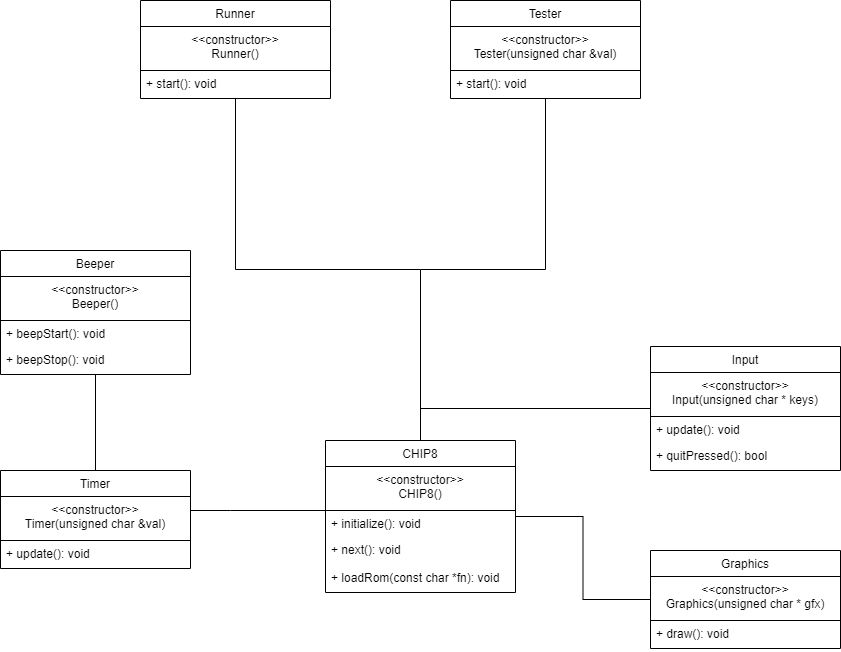
\includegraphics[width=\textwidth]{diagrams/class_diagram.png}
    \caption{Diagram klas}
    \label{fig:my_label}
\end{figure}

\section{Opis klas}
\begin{itemize}
    \item \verb+CHIP8+: Klasa odpowiedzialna za wykonywanie wgranego kodu, implementuje maszynę wirtualną interpretera CHIP-8.
    \item \verb+Beeper+: Klasa odpowiedzialna za wydanie jedynego dźwięku.
    \item \verb+Graphics+: Klasa odpowiedzialna za wyświetlanie grafiki.
    \item \verb+Input+: Klasa odpowiedzialna za wychwytywanie naciśnięć klawiszy.
    \item \verb+Timer+: Klasa odpowiedzialna za obsługę zegarów, których w CHIP-8 są dwa (60Hz)
    \item \verb+Runner+: Klasa odpowiedzialna za uruchomienie programu w trybie wykonywania zadanego kodu.
    \item \verb+Tester+: Klasa odpowiedzialna za uruchomienie programu w trybie testowym.
\end{itemize}{}

\chapter{Implementacja}
\pagestyle{fancy}

Interpreter CHIP-8 opiera się o maszynę wirtualną o specyfikacji:
\begin{itemize}
    \item dwubajtowy rejestr aktualnej instrukcji (\verb+unsigned short opcode+)
    \item 4KiB pamięci (\verb+unsigned char memory[4096]+)
        \begin{itemize}
            \item programy wgrywane są do pamięci na pozycji 0x200, poniżej jest przestrzeń zarezerwowana dla interpretera, w tym wypadku zawierać będzie wbudowane czcionki
        \end{itemize}
    \item 15 8b rejestrów ogólnego zastosowania (V0-VE) oraz jeden na flagę przeniesienia (VF)(\verb+unsigned char V[16]+)
    \item licznik programu (wartości od 0x000 do 0xFFF więc mieści się w 2B) (\verb+unsigned short pc+)
    \item rejestr indeksu (zakres taki jak w \verb+pc+) (\verb+unsigned short I+)
    \item 16sto poziomowy stos (\verb+unsigned short stack[16]+)
    \item wskaźnik stosu (\verb+unsigned char sp+)
    \item grafika
        \begin{itemize}
            \item 64x32
            \item monochromatyczna (piksel włączony lub wyłączony)
            \item rysowanie odbywa się przy pomocy spritów
            \item rysowanie odbywa się w trybie XOR, jeśli jakiś piksel zostaje wyłączony w trakcie rysowania ustawiana jest flaga VF, pozwala to na wykrywanie kolizji
        \end{itemize}
    \item obsługa 16 klawiszy (0x0-0xF) (\verb+unsigned char keys[16]+)
    \item dwa zegary
        \begin{itemize}
            \item dekrementują swoją wartość o zakresie 0x00-0xFF z częstotliwością 60Hz
            \item jeden z nich jest zegarem służacym do odliczania czasu
            \item drugi wywołuje dźwięk, jeśli ma niezerową wartość
        \end{itemize}
\end{itemize}

\clearpage

Po uruchomieniu programu odbywa się inicjalizacja rejestrów maszyny wirtualnej, zadany program wgrywany jest do pamięci maszyny od adresu 0x200. Po zakończeniu tego kroku, rozpoczyna się pętla emulacji:
\begin{enumerate}
    \item odświeżenie stanu maszyny
    \item pobranie instrukcji z pamięci
    \item zdekodowanie instrukcji
    \item wykonanie instrukcji
\end{enumerate}

Język CHIP-8 posiada 35 kodów operacyjnych (instrukcji), których spis znajduje się m.in. pod adresem: \href{https://github.com/mattmikolay/chip-8/wiki/CHIP\%E2\%80\%908-Instruction-Set}{https://github.com/mattmikolay/chip-8/wiki/CHIP-8-Instruction-Set}.

\end{document}